\documentclass[11pt,a4paper]{scrartcl}
\typearea{12}
\usepackage{graphicx}
\usepackage{pstricks}
\usepackage{amsmath}
\begin{document}


\section*{An introduction to programming}

Here is a simple programme for drawing a square; we will start with
this and try to make more complicated drawings.
\begin{center}
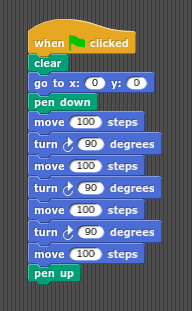
\includegraphics{basic_square.png}
\end{center}
Enter this and make sure it draws a square! One thing about this
program is that after it draws the square the arrow ends up pointing a
different direction to the direction it started in; can you fix this?
\begin{center}
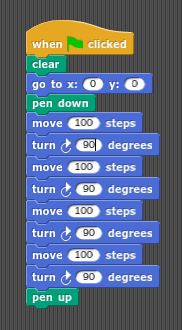
\includegraphics{basic_square_point.png}
\end{center}
Repeat
\begin{center}
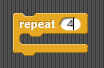
\includegraphics{repeat.png}
\end{center}
Can you use that to make the programme more succinct and readable? 
\begin{center}
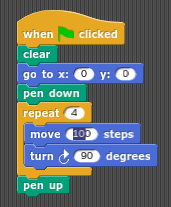
\includegraphics{repeat_square.png}
\end{center}


Now, look at this programme
\begin{center}
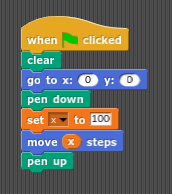
\includegraphics{variable.png}
\end{center}
Do the same to your square programme!
\begin{center}
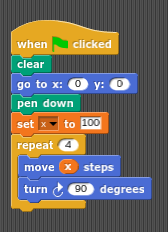
\includegraphics{variable_square.png}
\end{center}


This programme does something slighly more useful with a variable.
\begin{center}
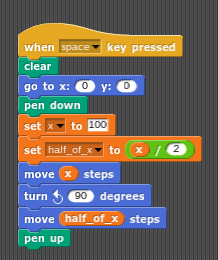
\includegraphics{line_half_line.png}
\end{center}
Try modifying your programme in a similar way so that it draws an
$n$-gon.
\begin{center}
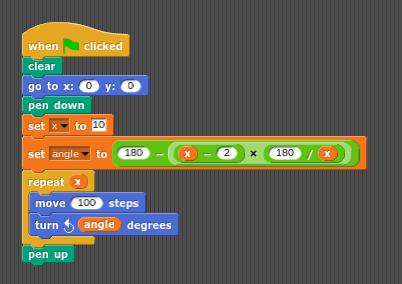
\includegraphics{n_gon.png}
\end{center}


In this programme the variable is changed in the \textsl{loop} so the
line is shorter each time:
\begin{center}
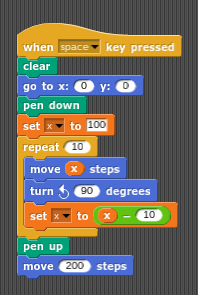
\includegraphics{spiral.png}
\end{center}
giving a spiral
\begin{center}

\includegraphics{spiral_pic.png}
\end{center}
Try modifying your programme in the same way so that you get smaller and smaller squares retreating into one corner, like this
\begin{center}
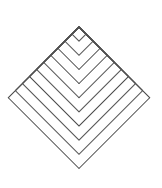
\includegraphics{repeat_squares_pic.png}
\end{center}
so
\begin{center}
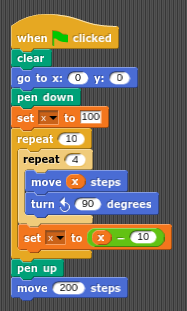
\includegraphics{repeat_squares.png}
\end{center}
If you want to you can try playing with you program a bit to give other patterns, like this
\begin{center}
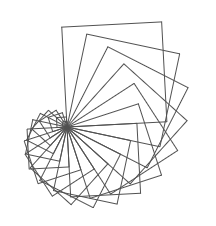
\includegraphics{squares_spiral_pic.png}
\end{center}
so 
\begin{center}
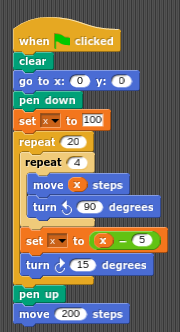
\includegraphics{squares_spiral.png}
\end{center}

This next programme draws a star;

This next programme draws a star
\begin{center}
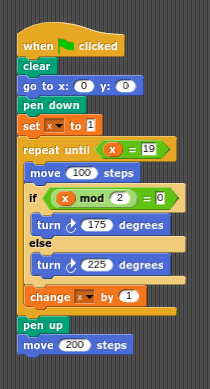
\includegraphics{star.png}
\end{center}

You can mess with programme a bit, maybe changing the angles or putting the whole thing in a loop to give something like this
\begin{center}

\includegraphics{rotating_star_pic.png}
\end{center}
so
\begin{center}
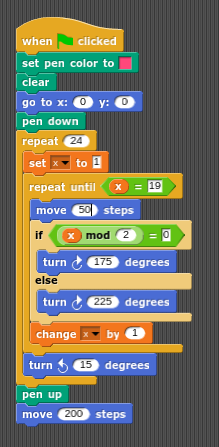
\includegraphics{rotating_star.png}
\end{center}

If anyone is finished with all of this maybe go on to blocks, for example
\begin{center}
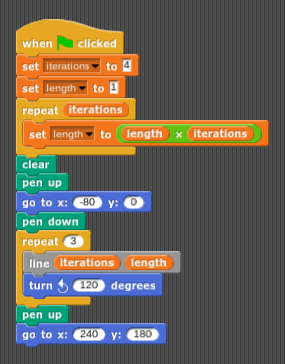
\includegraphics{koch.png}
\end{center}
with block
\begin{center}
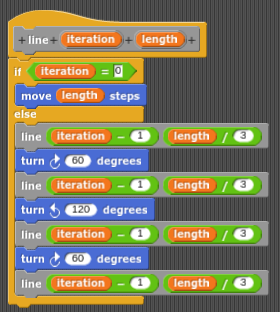
\includegraphics{koch_block.png}
\end{center}
draws
\begin{center}
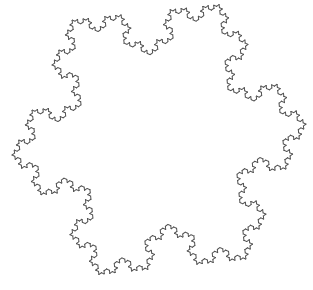
\includegraphics{koch_pic.png}
\end{center}



\end{document}
